\subsection{Das Heliumatom}
	\begin{align*}
		H = \left(\frac{\vec{p}^{(1)2}}{2m} - \frac{Z \alpha \hbar c}{r_1}\right)
		+ \left(\frac{\vec{p}^{(2)2}}{2m} - \frac{Z \alpha \hbar c}{r_2}\right)
		+ \frac{\alpha \hbar c}{|\vec{r}_1 - \vec{r}_2|}
	\end{align*}
Hierbei wurde die Spin Wechselwirkung vernachlässigt (warum auch immer), die beiden Terme in den Klammern sind $H^{(1)}$ und $H^{(2)}$, der Letzte ist $V_e(\vec{r}_1, \vec{r}_2)$, wir setzen $Z=2$ für 2 Protonen (obwohl $Z$ trotzdem immer wieder vorkommen wird).
	\begin{align*}
		\alpha_1 &= (n_1, \ell_1, m_1) & &\text{(weil Spin Ww vernachlässigt)} \\
		\vec{S} &= \vec{S}^{(1)} + \vec{S}^{(2)} & &\text{(Gesamtspin)}
	\end{align*}
	\begin{align*}
		\text{Gesamtspin }1& & \left(\vec{S}^2 \ket{\psi} = S(S+1) \hbar^2 \ket{\psi} \right) \\
		\ket{S, S_z} &= \ket{1 ,1} = \ket{+~+} \\
		\ket{S, S_z} &= \ket{1, -1} = \ket{-~-} \\
		\ket{S, S_z} &= \ket{1, 0} = \frac{1}{\sqrt{2}} \left( \ket{+~-} + \ket{-~+} \right)
	\end{align*}
Spinwellenfunktion ist symmetrsich. \\
$\Rightarrow$ Bahnwellenfunktion ist antisymmetrisch (\underline{Ortho-Helium})
	\begin{align*}
		\text{Gesamtspin }0& \\
		\ket{0 , 0} &= \frac{1}{\sqrt{2}} \left( \ket{+~-} - \ket{-~+} \right)
	\end{align*}
Spinwellenfunktion ist antisymmetrisch $\Rightarrow$ Bahnwellenfunktion ist symmetrisch (Para-Helium)

Gesamtwellenfunktion
	\begin{align*}
		\Psi(\vec{r}_1, \sigma_1 ; \vec{r}_2, \sigma_2) 
		&= \Psi(\vec{r}_1, \vec{r}_2) \chi (\sigma_1, \sigma_2) \\
		S = 1: \psi (\vec{r}_1, \vec{r}_2) &=
		\frac{1}{\sqrt{2}} 
		\left( \psi^{(1)} (\vec{r}_1) \psi^{(2)} (\vec{r}_2) 
		- \psi^{(1)}(\vec{r}_2) \psi^{(2)} (\vec{r}_1) \right) \\
		S = 0: \psi (\vec{r}_1, \vec{r}_2) &=
		\frac{1}{\sqrt{2}} 
		\left( \psi^{(1)} (\vec{r}_1) \psi^{(2)} (\vec{r}_2) 
		+ \psi^{(1)}(\vec{r}_2) \psi^{(2)} (\vec{r}_1) \right)
	\end{align*}
	\begin{align*}
		\text{mit } H^{(1)} \psi^{(1)} (\vec{r}) &= E^{(1)} \psi^{(1)} (\vec{r}) \\
		&\left(\text{bei Vernachlässigung von } V_e (\vec{r}_1, \vec{r}_2) \right) \\
		E_{\alpha_1 \alpha_2} &= E_{n_1 n_2} \approx 
		- \frac{1}{2} m c^2 Z^2 \alpha^2 
		\left( \frac{1}{n_1^2} + \frac{1}{n_2^2} \right)
	\end{align*}	
	\begin{align*}
		S = 0 &\Rightarrow n_1 = n_2 \text{ ist möglich immer.} \\
		S = 1 &\Rightarrow n_1 = n_2 \text{ für } n_1= 1
		(\Rightarrow \ell_1 = m_1 = 0 \Rightarrow \alpha_1 = \alpha_2) 
		\text{ ist verboten}
	\end{align*}
Grundzustandsenergie: 
	\begin{align*}
		E_{11} &\approx 2 E_1 = 2 Z^2 E_1 ( \overbrace{H}^{\mathclap{\text{Wasserstoff}}}) 
		= 8 E_1 (H) \approx -108,8 eV \\
		&( S= 0 (\text{Parahelium})) 
	\end{align*}
\underline{1.Anregung:}
	\begin{align*}
		E_{12} &\approx \left(1 + \frac{1}{4}\right) Z^2 E_1 (H) = 5 E_1(H) \approx -68,0 eV \\
		&(\text{möglich für Ortho- und Parahelium})
	\end{align*}
Betrachte $V_e(\vec{r}_1, \vec{r}_2) = \frac{\alpha \hbar c}{|\vec{r}_1 - \vec{r}_2|}$ als Störung
	
Grundzustand:
	\begin{align*}
		\Delta E_{11} &=
		\braket{ 1, 0, 0 ; 1, 0, 0| V_e | 1, 0 , 0; 1, 0 ,0 } & 
		&\text{also so:}\bra{n_1, \ell_1, m_1; n , \ell, m} \text{ usw.}\\
		&= \int \diff^3r_1 \diff^3r_2 |\psi_{100} (\vec{r}_1)|^2 |\psi_{100}(\vec{r}_2)|^2
		\frac{\alpha \hbar c}{|\vec{r}_1 - \vec{r}_2|} \\
		&\psi_{100} (\vec{r}) = \frac{1}{\sqrt{\pi}} 
		\left(\frac{Z}{a_B}\right)^{\frac{3}{2}} e^{-\frac{Zr}{a_B}}\\
		&= \frac{5}{4} \frac{Z \alpha \hbar c}{2 a_B} 
		= \frac{5}{4} Z \underbrace{\frac{mc\alpha^2}{2}}_{\mathclap{-E_1(H)}} 
		\approx 34 eV
	\end{align*}
	\begin{align*}
		E_{11} &= -108,8 eV + 34 eV + \ldots \approx - 74,8 eV \\
		\text{Experiment} &: -78,975eV (\text{Parahelium Grundzustand}) \\
		\Delta E_{1n} &\text{ mit } n>1 \\
		\psi (\vec{r}_1, \vec{r}_2) 
		&= \frac{1}{\sqrt{2}}
		\left( \psi_{100}(\vec{r}_1) \psi_{n \ell m}(\vec{r}_2) 
		\pm \psi_{100}(\vec{r}_2) \psi_{n \ell m} (\vec{r}_1) \right)
	\end{align*}
Das $``+''$ für Para-, das $``-''$ für Ortho-Helium.
	\begin{align*}
		\Delta E_{11} &=
		\int \diff^3 r_1 \diff^3 r_2 |\psi_{100} (\vec{r}_1)|^2 |\psi_{n \ell m} (\vec{r}_2)|^2
		\frac{2}{2} \frac{\alpha \hbar c}{|\vec{r}_1 - \vec{r}_2|} \\
		&\pm \int \diff^3 r_1 \diff^3 r_2 \psi_{100}^* (\vec{r}_1) \psi_{n \ell m}^* (\vec{r}_2)
		\psi_{100} (\vec{r}_2) \psi_{n \ell m} (\vec{r}_1)
		\frac{\alpha \hbar c}{|\vec{r}_1 - \vec{r}_2|} \\
		&= K_{n \ell} \pm A_{n \ell}
	\end{align*}
	\begin{align*}
		K_{n \ell} \geq 0 &: \text{Coulombenergie} & 
		&\text{Betrachte } n=2 \Rightarrow \ell = 0 \text{ oder } \ell = 1\\
		A_{n \ell} \geq 0 &: \text{Austauschenergie} \\
		\Delta E_{12} &= K_{2 \ell} \pm A_{2 \ell} &
		&\begin{aligned}
			&+ \text{ für Parahelium } 2^1 P, 2^1 S \\
			&- \text{ für Orthohelium } 2^3 P, 2^3 S
		\end{aligned}
	\end{align*}
	\begin{align*}
		K_{21} &= \frac{Z}{2} \alpha^2 m c^2 \frac{118}{243} \approx 13,2 eV \\
		A_{21} &= \frac{Z}{2} \alpha^2 m c^2 \frac{7}{12} \approx 15,9 eV
		,& A_{20} &= \frac{Z}{2} \alpha^2 m c^2 \frac{32}{729} \approx 0,6 eV
	\end{align*}
$\Rightarrow$ Ortho-Parahelium Energienieveauaufspaltung wegen des Pauli-Prinzips (Selbst wenn wir Spin Wechselwirkung in $H$ vernachlässigen) 

Spektroskompische Notation $n^{2 S + 1} \cdot L_J$

wobei $n=1,2,3$ und $L_J = S, P, D$ für $L=0, 1, 2$

	\begin{figure*} [h]
		\begin{center}
				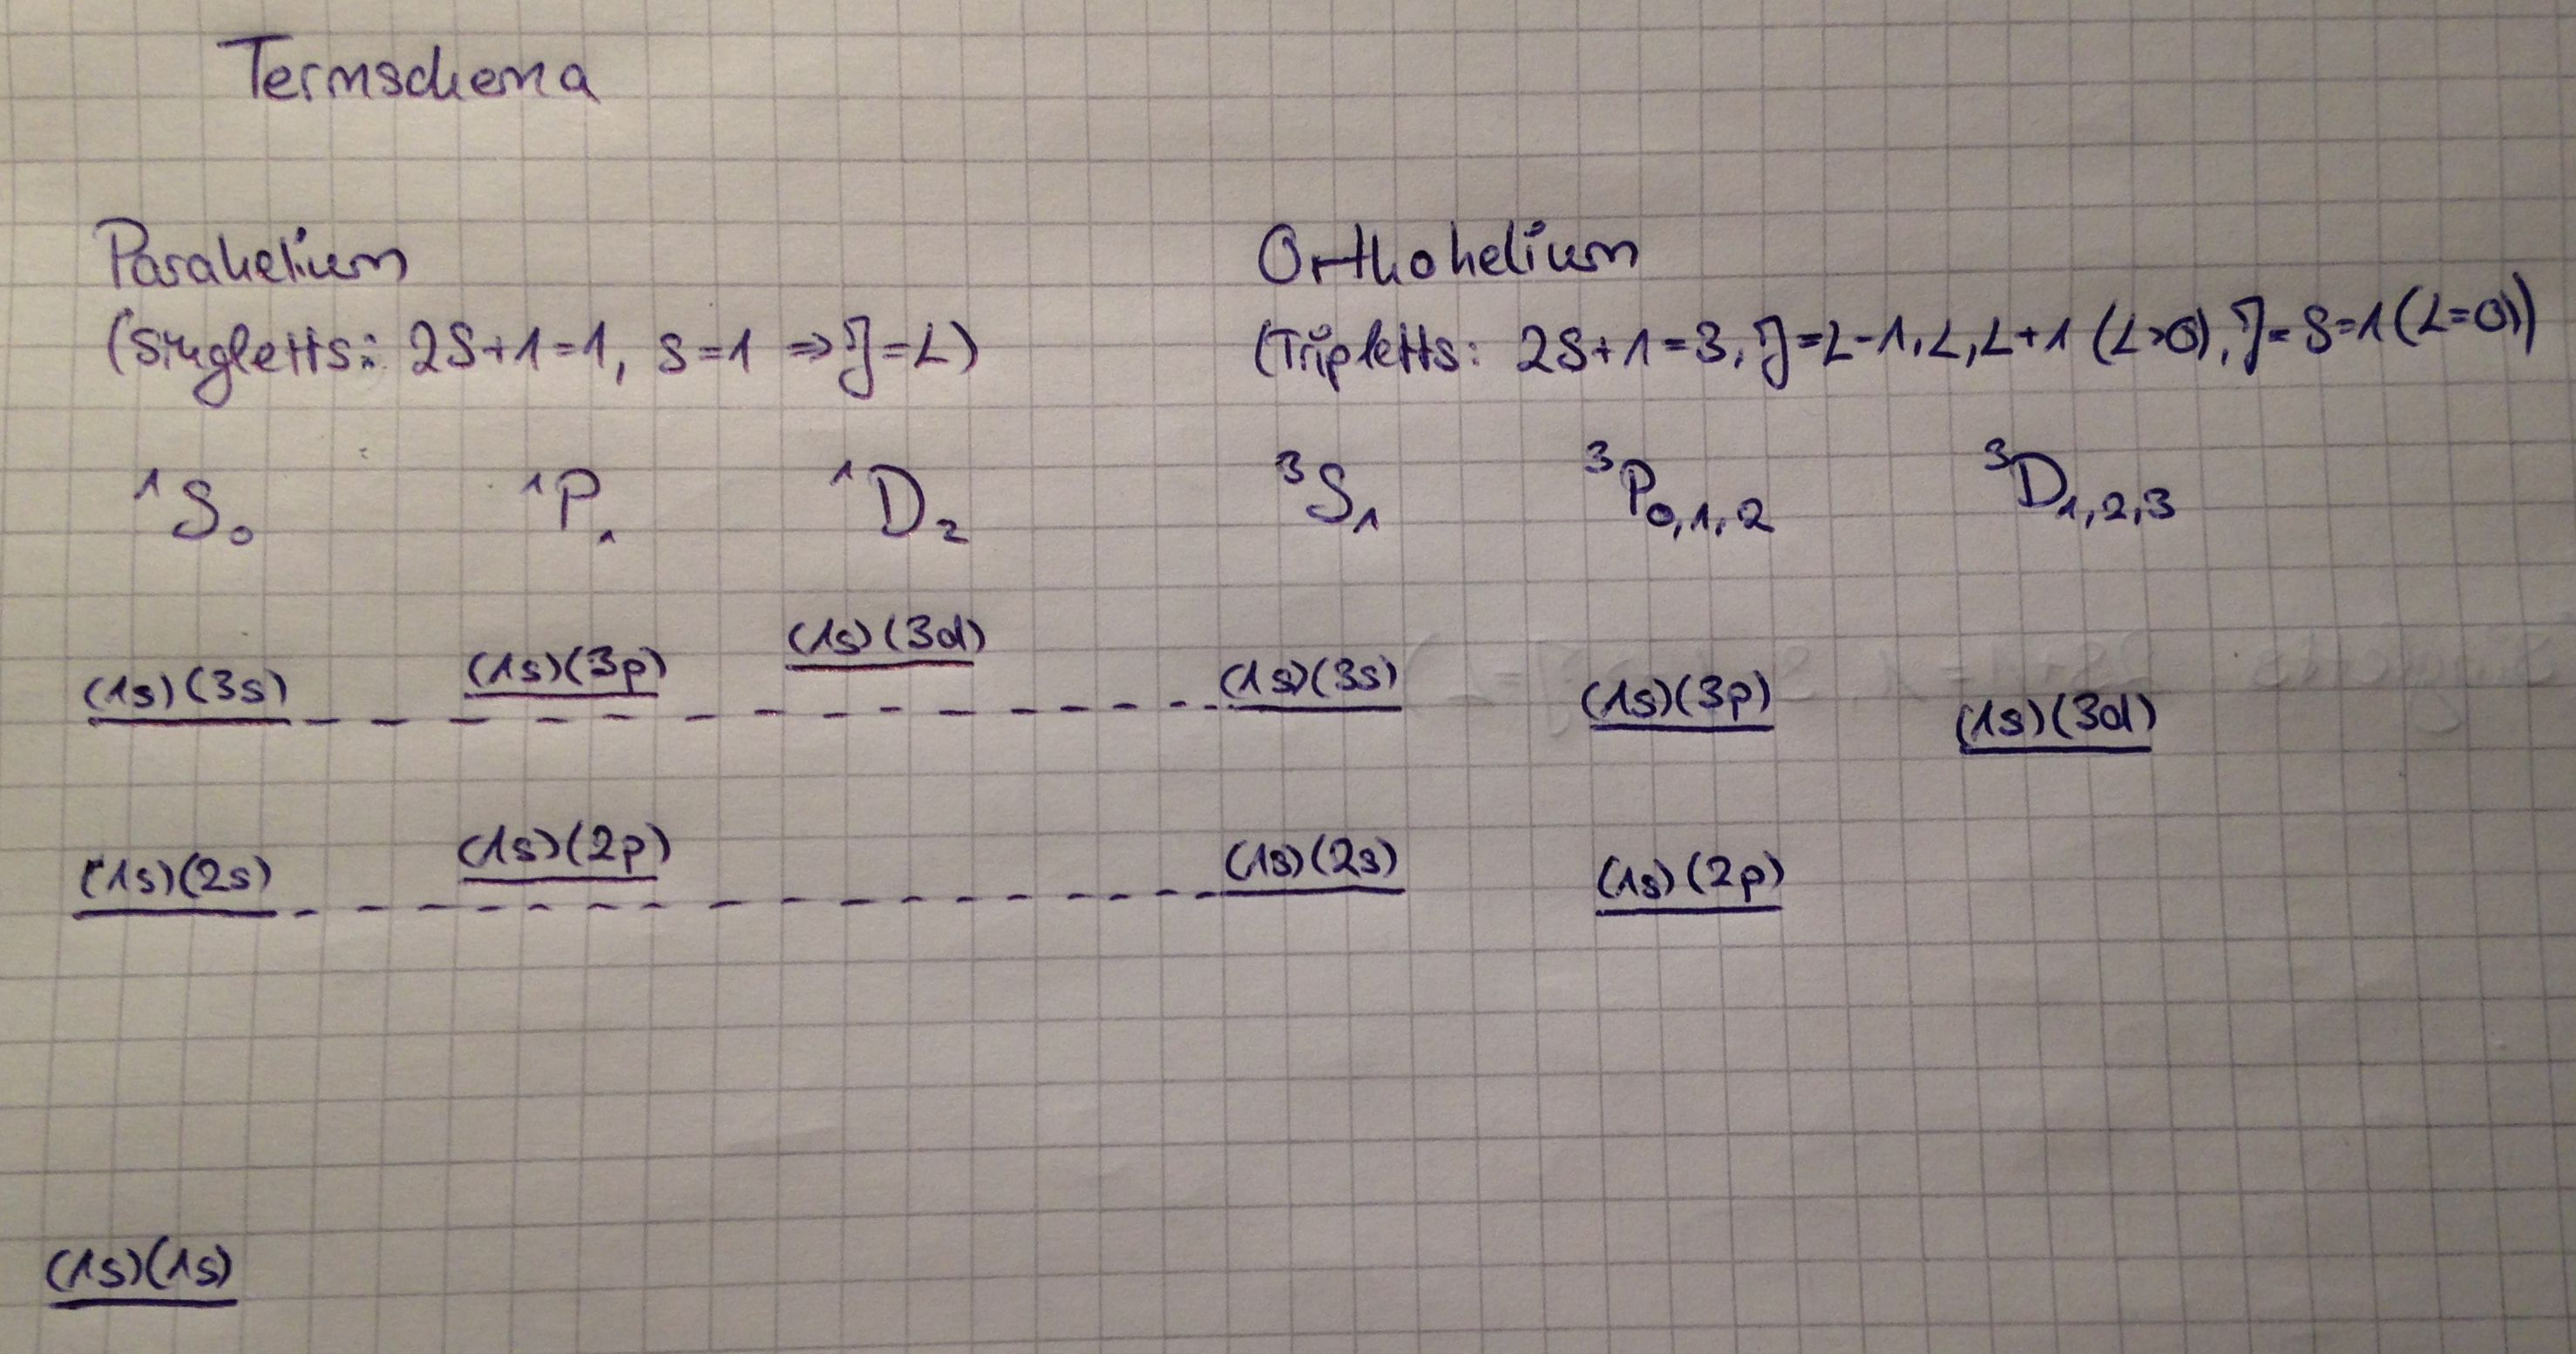
\includegraphics[width=\textwidth]{Termschema}
		\end{center}
	\end{figure*}

\subsection{Ritz-Variationsverfahren}
	\begin{align*}	
	\braket{\psi | H | \psi} &= \int \limits_\alpha\!\!\!\!\!\!\!\!\!\;\sum
	\braket{\psi | \alpha} E_\alpha \braket{\alpha | \psi} \\
	&\geq E_0 \int \limits_\alpha\!\!\!\!\!\!\!\!\!\;\sum |\braket{\psi | \alpha}|^2 
	= E_0 \braket{\psi | \psi}
	\end{align*}
	\begin{empheq}[box=\boxed]{align*}
		\Rightarrow \braket{\psi | H | \psi} &= E_0 \text{ für } \braket{\psi | \psi} = 1 \\
		\text{bzw. } E_0 &= \underset{\psi}{\mathrm{inf}} 
		\frac{\braket{\psi | H | \psi}}{\braket{\psi| \psi}}
	\end{empheq}
Betrachte eine nicht unbedingt normierte Testwellenfunktion, welche abhängt von kontinuierlichen Parametern $b_i$
	\begin{align*}
		\ket{\psi (b_1, \ldots, b_N)}& \\
		E(b_1, \ldots, b_N) &= 
		\frac{\braket{\psi (b_1, \ldots, b_N)|H|\psi (b_1, \ldots, b_N)}}{\braket{\psi (b_1, \ldots, b_N)|\psi (b_1, \ldots, b_N)}} \\
		E_{\text{min}} &= \underset{\{b_1, \ldots, b_N\}}{\mathrm{min}}
		E(b_1, \ldots, b_N) \geq E_0
	\end{align*}
Heliumatom
	\begin{align*}
		\text{Ansatz: } \psi_{100}(\vec{r}, Z^*)
		&= \frac{1}{\sqrt{\pi}} \left(\frac{Z^*}{a_B}\right)^{\frac{3}{2}} e^{-\frac{Z^* r}{a_B}}
	\end{align*}
Dies ist motiviert durch Wasserstoffwellenfunktion, aber mit ``effektiver'' Kernladung 
$Z* < Z = 2$, da das andere Elektron die Kernladung teilweise abschirmt.
	\marginpar{19.11.15}
	\begin{align*}
		H &= \underbrace{\frac{\vec{p}^{(1)2}}{2m} - \frac{Z^* \alpha \hbar c}{r_1}}_{\mathclap{*}}
		\underbrace{- \frac{(Z-Z^*)\alpha \hbar c}{r_1}}_{\mathclap{**}} \\
		&\underbrace{+ \frac{\vec{p}^{(2)2}}{2m} - \frac{Z^* \alpha \hbar c}{r_2}}_{\mathclap{*}}
		\underbrace{- \frac{(Z-Z^*)\alpha \hbar c}{r_2}}_{\mathclap{**}} \\
		&\underbrace{+ \frac{\alpha \hbar c}{|\vec{r}_1 - \vec{r}_2|}}_{\mathclap{V_e(\vec{r}_1, \vec{r}_2)}} + (\text{Spinabhängiger Term})
	\end{align*}
	\begin{align*}
		\braket{\psi_{100}(Z^*) | H | \psi_{100}(Z*)} 
		&= \underbrace{2E_1(Z^*)}_{\mathclap{*}} 
		\underbrace{- 2 \alpha \hbar c (Z - Z*) \erw{\frac{1}{r}}_{10}}_{\mathclap{**}}
	\end{align*}
Wobei * Grundzustandsenergie von $H$-Problem mit Kernladung $Z^* e$ und die $10$ beim Erwartungswert sind die $n \ell$ für Wasserstoff.
	\begin{align*}
		E_1(Z*) &= - \frac{1}{2} (Z^*)^2 m c^2 \alpha^2 ,&
		\erw{\frac{1}{r}}_{10} &= \frac{Z*}{a_B} \\
		\Rightarrow \braket{\psi | H | \psi} &= 
		-\frac{1}{2} m c^2 \alpha^2 
		\left( 2 (Z^*)^2 - 4 (Z^* - Z)Z^* \frac{5}{4} Z^* \right)\\
		&= \frac{1}{2} m c^2 \alpha^2 
		\left( 2 (Z^*)^2 - 8Z^* + \frac{5}{4} Z^* \right) & &\text{hier sind irgendwo Rechenfehler}
	\end{align*}
	\begin{align*}
		\frac{\partial \left(
			\frac{\braket{\psi | H | \psi}}{\braket{\psi | \psi}}
			\right)}{\partial Z^*}
		&= \frac{1}{2} m c^2 \alpha^2 \left( 4 Z^* - \frac{27}{4} \right) = 0 \\
		& \Rightarrow \boxed{Z^* = \frac{27}{16}} \\
		E_{\text{min}} &= - m c^2 \alpha^2 (Z- (Z - Z^*))^2 = -77,5eV
	\end{align*}
Zum Vergleich 

Störungstheorie, alles in $eV$ \\
	\begin{tabular}{c | c | c | c | c | c | c | c | c}
		Ordung & 0 & 1 & 2 & 3 & 4 & 5 & ``Exakt'' & Experiment \\
		\hline
		E & -108,832 & -74,822 & - 79,112 & -78,998 & -78,999 & -79,003 & -79,005 & -78,975
	\end{tabular}
Das Experiment weicht wegen der Wechselwirkungsterme, die wir vernachlässigt haben, ab.
	
	Ritz mit 2 Parametern $\psi \sim (1 + b_2 r) e^{-\frac{Z^* r}{a_B}} \leadsto -78,6eV$

\subsection{Atombau}

	\begin{tabular}{c c c c c c}
		$n$ & $\ell$ & Bezeichnung & Maximalzahl von $e^-$ & Besetzungsreihenfole & $Z$ \\
		\hline
		1 & 0 & $1s$ & 2 & 1 & 1-2 \\
		\hline
		2 & 0 & $2s$ & 2 & 2 & 3-4 \\
		  & 1 & $2p$ & 6 & 3 & 5-10 \\
		\hline
		3 & 0 & $3s$ & 2 & 4 & 11-12 \\
		  & 1 & $3p$ & 6 & 5 & 13-18 \\
		  & 2 & $3d$ & 10 & 6 & 19-30 \\
		\hline
		4 & 0 & $4s$ & 2 & 6 & 19-30 \\
		  & 1 & $4p$ & 6 & 7 & 31-36 \\
		  & 2 & $4d$ & 10 & 8 & 37-48 \\
		  & 3 & $4f$ & 14 & 10 & 55-80 \\
	\end{tabular}